\documentclass{style}

%%%%%% acronyms %%%%%%
\usepackage[acronym,toc]{glossaries}
\newacronym{UW}{UW}{University of Wisconsin}
%\newacronym{<++>}{<++>}{<++>}
\makeglossaries

\usepackage[printwatermark]{xwatermark}
\usepackage{xcolor}
\newwatermark[allpages,color=black!5,angle=45,scale=6,xpos=-40,ypos=40]{DRAFT}

%%%%%%%% cover info %%%%%%%%%%%%%%%
\title{Challenging Fuel Cycle Modeling Assumptions: Facility and Time Step Discretization Effects}
\author{Robert~W.~Carlsen, Paul~P.H.~Wilson}

\institute{University of Wisconsin - Madison, Department of Nuclear Engineering and Engineering Physics, Madison, WI 53706}
\submitter{Robert W. Carlsen}
\submitteraddress{229 N Midvale Blvd Apt 1, Madison, WI 53705}
\submitteremail{rwcarlsen@gmail.com}

% No more than three keywords, though each can be a phrase
\keywords{Nuclear Fuel Cycle, Simulation, Cyclus}

%%%%%%%%% includes and commands %%%%%%%%%%

\usepackage{graphicx}
\usepackage{placeins}
\usepackage{tabularx}
\usepackage{booktabs} % nice rules for tables
\usepackage{microtype} % if using PDF
\usepackage{xspace}
\usepackage{hyperref}
\usepackage{caption}
\usepackage{cite} % order citations correctly
\usepackage{float} % used to help position figures with the H modifier

\newcommand{\Cyclus}{\textsc{Cyclus}\xspace}%
\newcommand{\Cycamore}{\textsc{Cycamore}\xspace}%
\date{}

\myabstract{
Due to the diversity of fuel cycle simulator modeling assumptions, direct
comparison and benchmarking can be difficult.  In 2012 the Organisation for
Economic Co-operation and Development (OECD) completed a benchmark study that
is perhaps the most complete published comparison performed.  Despite this,
various results from the simulators were often significantly different because of
inconsistencies in modeling decisions involving reprocessing strategies,
refueling behavior, reactor end-of-life handling, etc.  This work identifies
and quantifies the effects of selected modeling choices that may sometimes be
taken for granted in the fuel cycle simulation domain.  Four scenarios are
compared using combinations of either fleet-based or individually modeled
reactors with either monthly or quarterly (3-month) time steps.  The scenarios
approximate a transition from the current U.S. once-through light water
reactor (LWR) fleet to a full sodium fast reactor (SFR) fuel cycle. The Cyclus
fuel cycle simulator's plug-in facility capability along with its market-like
dynamic material routing allow it to be used as a level playing field for
comparing the scenarios.  When under supply-constraint pressure, the four
cases exhibit noticeably different behavior.  Fleet-based modeling is more
efficient in supply-constrained environments at the expense of losing insight
on issues such as realistically suboptimal fuel distribution and challenges in
reactor refueling cycle staggering.  Finer-grained time steps also enable more
efficient material use in supply-constrained environments resulting in much lower
standing inventories of separated Pu.  Large simulations with fleet-based
reactors run much more quickly than their individual reactor counterparts.
Gaining a better understanding of how these and other modeling choices affect
fuel cycle dynamics will enable making more deliberate decisions with respect
to trade-offs such as computational investment vs.  realism.
}

%%%%%%%%%%%%%%%%%%%%%%%%%%%%%%%%%%%
\begin{document}

\section{Introduction}


The diversity of assumptions embedded within various fuel cycle simulators pose challenges for direct
comparison and benchmarking.  In 2012 the Organisation for
Economic Co-operation and Development (OECD) completed a benchmark study
\cite{oecd2012benchmark} that is perhaps one of the most complete published
comparisons performed.  Despite this, however, various results from the
different simulators were often significantly different because of inconsistent
modeling decisions involving reprocessing strategies, refueling behavior,
reactor end-of-life handling, etc.  This work attempts to identify and
quantify the effects of selected modeling choices relative to facility modeling
discretization (i.e., individual facilities vs. aggregate fleets) and time step
duration.  A better understanding of how these affect fuel cycle dynamics will
allow for making more deliberate decisions with respect to trade-offs such as
computational investment vs. realism.

This work identifies and quantifies the effects of selected modeling choices
that may sometimes be taken for granted in the fuel cycle simulation domain.
Four scenarios are compared using combinations of either fleet-based or
individually modeled reactors with either monthly or quarterly (3-month) time
steps.  Time step duration and the degree facility discretization are design
decisions that are handled in a variety of unique ways among nuclear fuel
cycle simulators, and a better understanding of their effects can serve to
increase confidence in results and can help make inter-simulator comparisons
more meaningful.  Reducing error and noise artifacts associated with modeling
decisions will provide a more stable foundation for understanding the
significance of external market, political, and social forces that often
dominate the industry in the real world.

\subsection{Motivation and Background}

Informal comparison of results from the VISION and Cyclus simulators when
running equivalent scenarios revealed some surprising discrepancies.  One of
the most apparent was a large difference in separated Pu levels between the
two simulators --- something that some in the DOE and nuclear community are
very sensitive to.  For one particular scenario, the Cyclus results also
showed no fuel shortages for reactors, while the VISION results indicated
noticeable shortages.  This observation prompted a closer investigation to
determine if the differences were caused by mistakes in simulator input, bugs
in the simulator(s), or differing modeling choices between the simulators.
This investigation eventually developed into this work which shows important
effects of some modeling choices that are operative in many fuel cycle
simulators.

Traditionally, many fuel cycle simulators have used a system dynamics approach
\cite{forrester_industrial_1961} to modeling. These simulators model several
\emph{stocks} representing isotopes or isotope groups that have quantities that change
over time because of \emph{flows} between them.  The flows are determined by equations
that are a function of the state of the system (i.e., the system's stocks).  A
constructed system is then solved in discrete or continuous time depending on
the limitations of the software and constraints imposed by the model.  In
system dynamics-based simulators, the number of stocks and potential flows between
them is generally a static property of the modeled system, making it somewhat
difficult to swap different reactor models in and out of the same scenario
without wiring them into the simulator manually.

System dynamics-based fuel cycle simulators generally use a collection of
stocks to represent the state of groups of like-facilities commonly referred
to as "fleets".  As the simulation steps through time, the levels of stocks
(e.g., reactor fresh fuel inventory, repository waste inventories, etc.) are
adjusted according to the calculated flow values.  Fuel cycle simulators that model
facility fleets built on a system dynamics foundation include VISION
\cite{jacobson_verifiable_2010}, DANESS \cite{van_den_durpel_daness_2009},
DYMOND, and ORION \cite{gregg_orion_2012} among
others.  In fleet-based modeling:

\begin{itemize}

    \item Groups of facilities (usually all facilities of a given type) are
        treated as a single, aggregate entity. Therefore, all facilities experience
        a single, identical history.

    \item Resource flows are modeled as continuous, within the limitations of time
        step discretization.  Therefore, material is acquired and discharged in
        uniform amounts at every time step.

\end{itemize}

This work investigates in detail some differences between fleet vs. individual
reactor modeling.  The difference between these two modeling styles in terms
of their effects on output of fuel cycle simulators in general is not well
known. This analysis is designed to provide both quantitative and
qualitative insight about how fleet-based continuous flow models differ from
individual facility discrete flow models.

Many fuel cycle simulators step through time in discrete steps.  The duration
of a single time step can have significant impact on the dynamics of a
simulation.  The time step duration can affect the magnitude of individual
material transfers between facilities and correspondingly affects the noise
level in facility material inventories and flows.  It can also act as a
minimum bound for outage durations and is a minimum bound in general for state
changes within the entire system. The effects of the time step duration are
also investigated together with fleet vs. facility modeling.

Questions of interest include:

\begin{itemize}

    \item What effects drive differences in fleet-based and individual-based
        facility modeling?

    \item How does changing the time step duration affect simulations?

    \item Does the impact of changing time step duration differ in fleet-based
        and individual-based facility modeling?

\end{itemize}

\subsection{Cyclus}

One of the major motivations for the development of the Cyclus fuel cycle
simulator \cite{cyclus_2015} was creating a simulation environment that is
more expressive than more traditional fuel cycle simulators.  Cyclus was
designed with a plug-in style architecture that allows different models for
facility types, known as \emph{archetypes}, to be swapped in and out easily.
While the reactor archetypes used in this analysis do not implement
internal physics calculations, plug-in archetypes such as Bright-lite
\cite{flanagan_bright-lite_2014} have been developed for Cyclus that provide
varying degrees modeling fidelity.
% response to technical comment 2.

As a Cyclus simulation walks through each time step, facilities engage in a
market-like dynamic resource exchange (DRE).  They broadcast requests for
material and potential supplying facilities respond with bids. The requesting facilities then
express preferences between all their bids, and the DRE then generates a network
flow problem that is optimized to resolve which transactions actually occur.
The plug-in architecture combined with the DRE creates a powerful and flexible
environment for the natural comparison of different modeling paradigms.
Cyclus' module plug-in based architecture in concert with its DRE has the ability to
model fleet-based facilities.  Additionally, Cyclus can model
facilities individually with discrete flows enabling the investigation of
real-world effects such as competition, reactor cycle staggering,
and individual reactor outages. 

Cyclus was designed to operate natively in Unix/Linux type environments with
flexible and scriptable usage and input file format.  Cyclus stores its
comprehensive output data in a powerful open-source database format.  In addition
to information about material flows and facility deployments, Cyclus'
single-file database contains the simulation input file, version information
about the archetypes used in a simulation, the version of Cyclus used to run
the simulation, and the installed versions of Cyclus dependencies. This and
other features of Cyclus lend themselves well to automation, research
provenance and reproducibility, and large-scale computing.

\section{Methodology}

Two particular design choices are selected for investigation: time step
duration and facility discretization.  A single fuel cycle transition scenario
is run in a set of simulations using combinations of the time step duration
and facility discretization  --- four four different cases:

\begin{enumerate}

    \item \emph{Case MI}: \underline{M}onthly time steps with \underline{I}ndividual reactor modeling
    \item \emph{Case MF}: \underline{M}onthly time steps with \underline{F}leet reactor modeling
    \item \emph{Case QI}: \underline{Q}uarterly (3-month) time steps with \underline{I}ndividual reactor modeling
    \item \emph{Case QF}: \underline{Q}uarterly (3-month) time steps with \underline{F}leet reactor modeling

\end{enumerate}

%% response to technical comment 1.
These four cases span a spectrum of fidelity with one end being more realistic
(i.e., smaller time steps, individual facilities) and the other being more
appropriate for scoping studies (i.e.,  larger time steps, fleet facilities).
Conducting this analysis involved developing some additional capability
in/around Cyclus.  Three primary pieces to the methodology are:

\begin{itemize}

    \item A fleet-based reactor model.

    \item A simulation scenario with both initial conditions and transition
        details.

    \item Theory and metrics for comparing differences between the four cases.

\end{itemize}

Because the standard package of archetypes included with Cyclus does not
include a fleet-based reactor model, one was necessarily developed. A
simulation scenario was created that is roughly based on prior and ongoing
work in the Department of Energy (DOE) fuel cycle options campaign.  A few
phenomena related to the different modeling choices in each of the four cases
are identified and used as a basis for comparison.  These are
described in more detail in the following sections.

\subsection{Fleet Reactor Implementation}

A fleet reactor archetype was created for Cyclus.  Although the modeling of
individual, discrete facilities was a motivation for Cyclus, its flexibility
makes it relatively straightforward to create plug-in archetypes to model
anywhere along the spectrum from individual, discrete facilities to continuous
flow fleet facilities.  In order to contrast well with the individual,
single-facility granularity modeling that is part of the standard Cyclus
archetypes, a fleet archetype was created for this work with aggregate
facility behavior and continuous flow.  Although it would certainly be
interesting to compare many intermediate levels of facility discretization
(e.g., 1-reactor groups, 10-reactor groups, single-fleet, etc.), such a
detailed analysis is beyond the scope of this work.
% address technical comment 14

The fleet reactor, although a single entity modeling many reactors, is
actually designed to look like many individual reactors to the Cyclus
simulator kernel. This "trick" allows other plug-ins for managing facility
deployments to transparently work with the fleet reactor without having to
know anything about the fleet paradigm.  The fleet reactor has several
important characteristics described below:

\begin{itemize}

    \item Reactor capacity is deployed and retired in increments of single
      reactor units, each capable of producing power $P_r$ (e.g., 1 GWe
      LWRs).  $N_{r}$ reactors are deployed at any time capable of producing
      up to $P_r \cdot N_r$ power.

    \item In the event of fuel shortages, the number of reactors that can
      operate is modeled as

      \begin{equation}
        N_{o} = N_{r} \cdot \frac{C_{inv}}{C_{cap}},
        \label{eqn:operating-reactors}
      \end{equation}

       where $C_{inv}$ is the total amount of fuel in all reactor cores (kg),
       and $C_{cap}$ is the total fuel capacity for all reactor cores (kg).

    \item Material is discharged from the fleet's reactor cores continuously
        (every time step) according to the following equation:

        \begin{equation}
            D =
            \frac{B}{L} \cdot N_{o} =  \frac{B}{L} \cdot N_{r}\cdot \frac{C_{inv}}{C_{cap}}
            \label{eqn:fleet-discharge}
        \end{equation}

        $D$ is the discharge rate (kg per time step), $B$ is the batch size
        (kg) for a single reactor's batch, $L$ is the cycle length (including
        refueling time) in time steps.  In the event of fuel shortages, the
        discharge rate is reduced because some reactors are not operating.

    \item Refueling occurs continuously with as much fresh fuel as is
        available up to the total amount to fill all reactor cores in the
        fleet.  No extra fuel is kept on-hand --- it is all ordered
        just-in-time.

    \item Generated power at any time step, $P_G$, is based on the number of
      operating reactors:

      \begin{equation}
        P_{G} = P_r \cdot N_o = P_r \cdot N_r \cdot \frac{C_{inv}}{C_{cap}}
      \end{equation}

    \item When a reactor in the fleet is retired, a full core of material is
        discharged --- even if there is some fraction of the fleet with unfueled
        cores.
        
\end{itemize}

One characteristic of this fleet reactor implementation is that it has perfect
fuel sharing and perfect cycle staggering among the individual reactors it
models.  The first discharge of spent fuel begins immediately on
the first time step of operation rather than after a complete refueling cycle.
Fuel shortages also only cause proportional loss of capacity rather than
whole-reactor quantized shutdown.  The full implementation of the fleet-based
reactor is publicly available for download and use \cite{Carlsen2015}.

\subsection{Scenario Description}

The chosen scenario approximates a transition from the current once-through light water
reactor (LWR) fleet to a full sodium fast reactor (SFR) fuel cycle within evaluation group 23 (EG-23)
in the DOE's Advanced Nuclear Fuel Cycle Options report
\cite{wigeland_nuclear_2014}. Scenario and transition details were patterned
after ongoing work by the DOE in their Fuel Cycle Options campaign.
%% Not sure if we should make such an explicit reference to the ongoing FCO
%% transition work until they publish something. On one hand, it reveals
%% things they are secretive about. On the other hand, we should give them due
%% credit.


The scenario starts with 100 LWRs and follows an exponential curve with a 1\%
annual growth rate for 200 years.  The decommissioning of the initial 100
reactors is staggered over years 15 to 55.  Fresh fuel for LWRs is provided directly from enrichment with infinite supply and throughput. In year 35, fast reactors become available for
deployment and no more thermal reactors are built.  LWR spent fuel separations
begins in year 15 with 2,000 MTHM/yr capacity and increases to 3,000 MTHM/yr in
year 25.  Fast reactor spent fuel separations and fuel fabrication have
infinite capacity.  All spent fuel is stored/cooled for 7 years before it becomes
available for separation: 5 years for cooling and an additional 2 years to approximate non-instantaneous separations and fabrication times. Figure \ref{fig:flow} shows the material flow
relationships between the facilities.  Compositions used for the simulations
were simple containing $^{238}U$, $^{235}U$, $^{239}Pu$, $^{241}Am$,
and small quantities of a few lanthanides.  Full composition details can be
found in the Cyclus input files used \cite{Carlsen2015}.

\begin{figure}[!h]
    \centering
    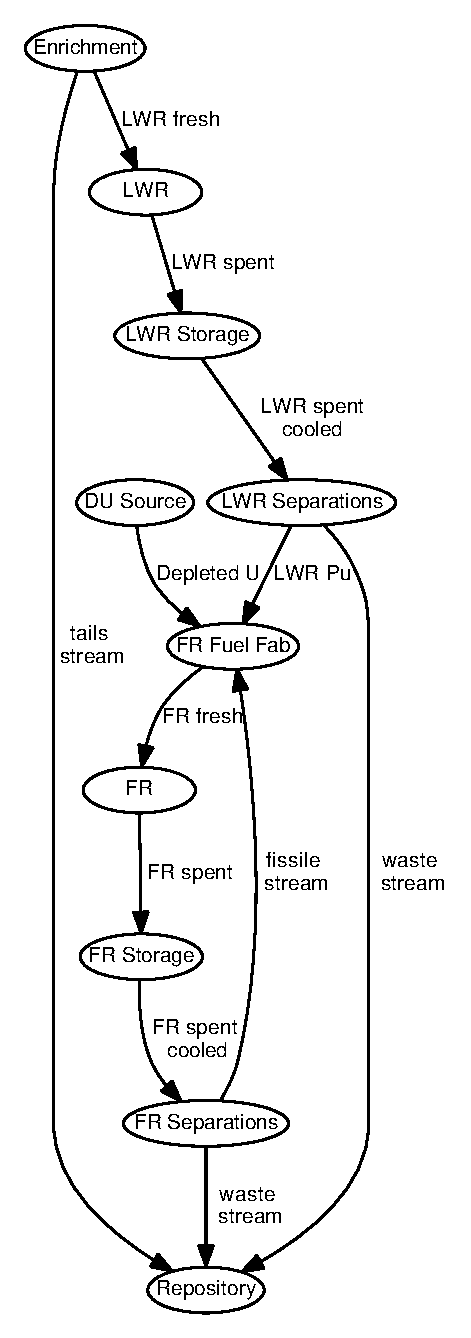
\includegraphics[keepaspectratio=true,width=0.45\textwidth,height=.89\textheight]{exp2/flow.eps}
    \caption[Material flow paths]{
        Material flow paths between facility types. The DU source is separate
        from enrichment tails for modeling simplicity, although enrichment
        tails could be used for added realism.  The primary fissile isotope in
        the fissile separations stream is $_{239}Pu$.
    }
    % response to technical comment 9
    \label{fig:flow}
\end{figure}

%% is it worth waiting until the 1.4 release?  Citing an ambiguous pre-release makes
%% this a little harder to reproduce.
A pre-release of Cyclus version 1.4 was used for this analysis.  A standard library of facility plug-ins, Cycamore, is provided with Cyclus.
Like Cyclus, a pre-release of Cycamore version 1.4 was used.  A custom storage facility archetype was
developed because Cycamore did not yet provide one.  Code for the fleet reactor and
storage archetypes is publicly available and can be downloaded \cite{Carlsen2015}. The standard Cycamore reactor archetype
was used for both LWR and SFR reactor types in cases MI and QI.  Correspondingly
the custom fleet-based reactor archetype described earlier was used for both reactor
types in cases MF and QF.  Additional configuration for the reactor types is
shown in Table \ref{tab:reactors} (cycle length includes the refueling outage).

\vspace{2mm}

\begin{table}[h]
    \caption{Reactor Facility Parameters}
    \centering
    \begin{tabular}{ |r | c c | }
        \hline                       
            & LWR & SFR \\
        \hline                       
        Lifetime (yr)         & 80 & 80 \\
        Cycle length (months) & 18 & 15 \\
        Batch size (kg)       & 29,565 & 8,025 \\
        Batches per core      & 3 & 5 \\
        \hline                       
    \end{tabular}
    \captionsetup{justification=centering}
    \label{tab:reactors}
\end{table}

The described scenario is used as closely as possible in each of the four
cases with appropriate adjustments for case-specific differences (e.g., monthly
vs. quarterly time steps).  Invariants preserved with respect to reactor
behavior between all four cases are shown in Table \ref{tab:invar}.  Table
\ref{tab:reactor-detail} shows the computed/selected configuration for both
LWR and SFR reactor types that was used in Cyclus input files for all four
cases.

\begin{table}
    \captionsetup{justification=centering}
    \caption{Reactor Parameter Invariants}
    \centering
    \begin{tabular}{ |r | c c | }
        \hline                       
                                                                             & LWR      & SFR      \\
        \hline                       
                                                                             &          &          \\
        Discharge Rate ($\frac{\text{kg} \cdot \text{HM}}{\text{month}}$)           & 1,642.5   & 535      \\
                                                                             &          &          \\
        Burnup  ($\frac{\text{MWe} \cdot \text{month}}{\text{kg} \cdot \text{HM}}$) & 0.547945 & 0.672897 \\
                                                                             &          &          \\
        Effective Power  ($\text{MWe}$)                                      & 900      & 360      \\
                                                                             &          &          \\
        Core Size  ($\text{kg} \cdot \text{HM}$)                                    & 88,695    & 40,125    \\
                                                                             &          &          \\
        \hline                       
    \end{tabular}
    \label{tab:invar}
\end{table}

\begin{table*}
    \centering
    \captionsetup{justification=centering}
    \caption{Selected Reactor Parameters by Case}
    \begin{tabular}{ |r | c c | c c | }
        \hline                       
                                          & \multicolumn{2}{c |}{LWR}       & \multicolumn{2}{c |}{SFR} \\
                                          & Cases MI, QI & Cases MF, QF & Cases MI, QI & Cases MF, QF  \\
        \hline                       
        Cycle length (months)             & 15        & 18                & 12        & 15 \\
        Refueling outage (months)         & 3         & 0                 & 3         & 0 \\
        Batch size ($\text{kg} \cdot \text{HM}$) & 29,565    & 29,565            & 8,025     & 8,025 \\
        Power capacity (MWe)              & 1,080     & 900               & 450       & 360 \\
        \hline                       
    \end{tabular}
    \label{tab:reactor-detail}
\end{table*}

In each of the four cases, the initial 100 LWRs are modified to have a
zero-length refueling outage with an explicit 900 MWe net power output
capacity.  Because the individual reactor model does not have any way to start
a reactor mid-cycle, this is a modeling trick that was done to avoid having
all initial LWRs refuel at the same time.  This adjustment serves to improve
the realism associated with the effects being investigated (i.e., fleet-average
power generation) even though it is unrealistic in other ways.
% response to technical comment 11

The parameters for each case were also selected to keep capacity factors for
individual reactors very roughly around 90\%, although they are actually
closer to 80\% because of integer variable constraints on the case MI and QI
reactor configuration.  

% response to technical comment 12
Instead of annual deployments, a longer 21-month deployment period is used
because it provides better natural staggering for the reactor refueling
cycles. The 630-month lowest common multiple (LCM) for 21-months (deployment
period), 15 months (SFR cycle), and 18 months (LWR cycle) is much larger than
the 180-month LCM when using a 12-month build period providing a more even
power generation profile.  The same deployment schedule is used for all four
cases; power capacity is built along a curve starting at 100 GWe in year zero
following the 1\% exponential growth curve.  Although many alternate
deployment schedules exist that avoid SFR fuel shortages (e.g., a more gradual
shift toward SFRs), this particular schedule is deliberately chosen because it
causes significant fuel shortages.  This is done in order to force the
simulation and facility models into more extreme circumstances in order to
expose behavioral differences among the design choices investigated.
% response to general comment paragraph
% response to technical comment 13

All input files and other assets used in the analysis for each of the four
cases are publicly available for download and use \cite{Carlsen2015}.

\subsection{Modeling Effects}

There are various low-level phenomena that have potential to affect the larger
outcome of simulations with respect to facility discretization and time step
modeling decisions. Several effects arising from these different modeling
choices are present in many fuel cycle simulators to varying degrees.  Some of
these effects are described in detail below.

One difference between the fleet and individual facility modeling is the
\emph{quantized shutdown effect}.  If a fleet-based reactor modeling 3-batch
cores is short one half batch of fuel, it will produce $\frac{2.5}{3}\cdot P_r$
of power for that time step where $P_r$ is the power capacity of a single
reactor of the fleet (e.g.,~1000~MWe).  If an individually modeled reactor is
short one half batch of fuel, then it will produce no power ($0 \cdot P_r$) that
time step.  Time step duration can amplify this effect.  For both fleet and
individual reactor modeling, power goes offline in full time step increments.
Consider an example of a 3-batch reactor with a fuel shortage of $\frac{1}{2}$ batch of
fuel that would be resolved in 1 month.  Depending on the modeling choice, each reactor
would produce the following amounts of energy over a 3 month period:

\begin{itemize}
  \item case \emph{QF}: $\frac{2.5}{3} \cdot 3 \text{ mo} \cdot P_r = 2.5P_r$
  \item case \emph{MF}: $[\frac{2.5}{3} \cdot 1 \text{ mo} + 1 \cdot 2
    \text{mo}] \cdot P_r = 2.83P_r$
  \item case \emph{QI}: $0 \cdot 3 \text{ mo} \cdot P_r = 0$
  \item case \emph{MI}: $(0\cdot 1 \text{ mo} + 1 \cdot 2\text{ mo}) \cdot P_r = 2 P_r$
\end{itemize}

Quantifying this effect directly is difficult.  One way of observing
it is to compare fleet reactor scenarios that have different time step
durations (i.e., cases MF and QF).  Because the fleet reactors have perfect fuel
sharing (described below) and no noise from refueling outages, differences observed will
partly be a result of quantized shutdown.

Individually modeled reactors each have their own refueling cycles.  Depending
on how the refueling cycles and outages are staggered, power production can
vary significantly.  For example, if all reactors refuel at the same time,
then all reactors are offline at the same time.  This is referred to as the
\emph{cycle staggering effect} and does not occur in fleet-based reactor
models.  An example of poor cycle staggering is shown in Figure
\ref{fig:sync-cycle}.  This effect can be naturally observed as the
fluctuations in the difference between deployed power capacity and generated
power.  The figure shows power jumping above and below the installed net
capacity (includes capacity factor) from time step to time step depending on
how many reactors are online/offline together.

Poor reactor cycle staggering can also cause spikes of material supply and
demand that can lead to suboptimal resource utilization.  Consider a fuel
fabrication facility that receives requests for new batches for every reactor
all at once.  The reactors draw out inventory from the fuel fabrication
facility together in a large quantity of orders.  If the fabrication facility
does not have enough material on hand, some number of reactors will need to
wait until enough fuel can be fabricated.  Avoiding such
constraints would require the fabrication facility to maintain suboptimally
large on-hand inventories as a contingency.  Even with infinite material
availability, poor staggering can result in supply constraints caused by
finite facility throughput. Even if the fuel fabrication facility above has
infinite material supply that it can keep on hand, it might not be able to
fabricate fuel for all reactor requests all at once even though it has
sufficient capacity if they request fuel uniformly over time.

\begin{figure}[h]
    \centering
    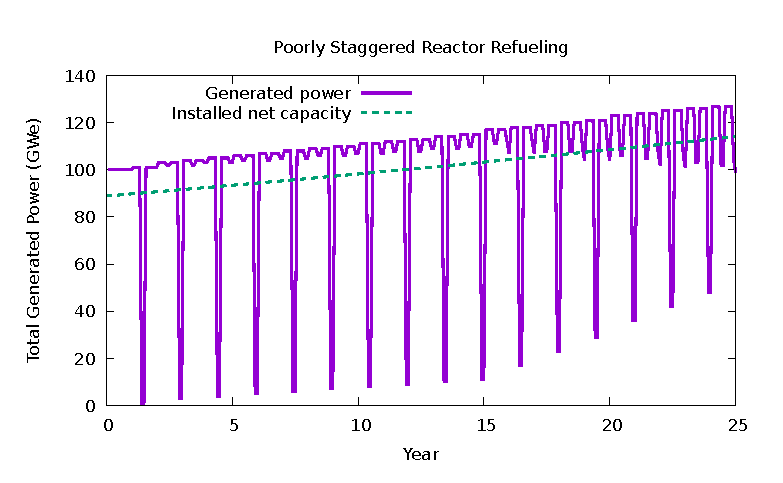
\includegraphics[width=1.0\columnwidth]{exp2/sync-cycle.eps}
    \caption[The cycle staggering effect]{
        In this scenario, reactors are deployed annually with a refueling cycle
        length (including outage) of 18 months.  As a result, all reactors deployed
        every 3rd year refuel together.  All initial 100 LWRs start out with
        their cycles synced as well.
    }
    \label{fig:sync-cycle}
\end{figure}

Another difference between fleet-based and individual facility modeling
involves fuel sharing.  Power production by a group of individual reactors for
a fixed amount of fuel shortage may vary depending on how available fuel is
distributed.  This is illustrated in Figure \ref{fig:fuel-sharing}.  A system
being short 3 batches might mean that one reactor has no batches and is not
operating or that 3 reactors are each missing a single batch.  This is
referred to as the \emph{fuel sharing effect}.  Fleet reactors, by design,
have perfect fuel sharing --- all fuel is distributed so that the minimum
possible amount of capacity is offline during shortages.  The most correct
measure of fuel sharing inefficiency is the difference between the actual
generated power and the maximum amount of power that could have been generated
among all possible fuel distribution alternatives.  This is difficult to
actually compute. One possible approximation is to count the number of fresh
fuel batches distributed to reactors that ended up not having enough fuel to
operate (i.e., a full core) that time step.  This approximation assumes that
every "wasted" batch of fuel, could have been given to a reactor that only
needed one batch to operate.  Equation \ref{eq:badshare} describes such an
approximation.

\begin{equation}
    N_{wasted}(t) = \sum\limits_{r \in R_t} \left(H[t-(\tau(t,r) + \Delta\;t_{out})] \cdot [1-O(t,r)]  \sum\limits_{t'=F_{prev}(t,r)}^{t} N_b(t',r) \right)
    \label{eq:badshare}
\end{equation}
%% What is the value of this function during a normal refueling outage,
%% immediately before S_(sched)(t)?  It seems you need another Heavyside
%% function to drop this back down to an expected value of 0 again.
%%
%%          ___________________
%%          |                 |
%%  ________|                 |_____________

\noindent
where $R_t$ is the set of all reactors, $H$ is the Heaviside function,
$\tau(t,r)$ is the beginning of the most recent refueling outage of reactor $r$ before $t$,
$\Delta\; t_{out}$ is the normal refueling outage duration, $F_{prev}(t,r)$ is
the start of the most recent refueling outage for reactor $r$ before or on
time $t$, $O(t,r)$ is 1 if reactor $r$ is producing power at time $t$ and zero
otherwise, and $N_b(t,r)$ is the number of new fuel batches received by
reactor $r$ since time $t$.

\begin{figure}[h]
    \centering
    \includegraphics[width=0.8\columnwidth]{exp2/fuel-sharing.pdf}
    \caption[The fuel sharing effect]{
        A simple diagram showing effects of constrained fuel supply
        distribution choices. In both cases A and B, reactor 1 needs 3 new
        fuel batches to operate and reactors 2 and 3 each need 1 fresh batch.
        In case A, the two batches are given to reactors 2 and 3, resulting in
        reactor 1 remaining offline. In case B, the available fuel batches are
        given to reactor 1 resulting in all three reactors being offline.
    }
    \label{fig:fuel-sharing}
\end{figure}


One important phenomenon related to time step duration is the \emph{inventory
drawdown effect}.  Increasing time step duration reduces the frequency over
which refueling can occur, resulting in larger impulse drawdown on
inventories. This by itself is not problematic because this is balanced by
correspondingly larger inventory top-up quantities.  However, another
component of this effect is the simultaneity of incoming and outgoing material
flows on a given time step.  Within a particular time step facilities do not
know about incoming material when they make commitments for outgoing material.
For longer time steps, larger incoming quanta of material are not available
for making offers. In general longer time steps create a need for larger
floating inventory buffers in order to avoid material shortages.  Another
aspect of this effect is that at least one time step is required for a
material object to move between two facilities. Larger time steps result in
longer minimum bounds on time to traverse paths between facilities. Although
direct measures of this effect are difficult, some of its consequences (e.g.,
higher standing inventories during shortages) can be quantified by comparing
scenarios with different time step durations (e.g.,  cases MF and QF).

There are also performance differences between the two modeling paradigms.  A
single 200 year simulation with several hundred fleet-based reactors takes
about 2 seconds to run on a computer with an Intel Core(TM) i7-4770 3.40GHz CPU where the same simulation
using individual reactor facilities takes about 20 seconds.  This order of
magnitude difference is an important trade-off to keep in mind when doing fuel
cycle analysis in general, particularly when considering optimization or
sensitivity studies where running thousands or millions of simulations may be
desirable.  The time step duration has less impact on performance because the
amount of work being done in the simulation is similar; in the monthly time
step cases most facilities (i.e., all reactors) only perform actions every
refueling cycle rather than every time step.

\section{Results}

\subsection{Power Production}

Figure \ref{fig:power} shows an overall view of the generated power over time
for each of the four cases.  Figure \ref{fig:power-rel} normalizes the Figure
\ref{fig:power} curves to the expected exponential power curve magnifying some
interesting differences between the four cases.  For the first 100 years, the
four cases behave somewhat similarly, although the individually modeled
reactors in cases MI and QI actually go offline and back online for refueling
causing more variance.  Around year 100, a fuel shortage begins and more
significant differences between the four cases become apparent. This fuel
shortage lasts until about year 140. The power generated in case QF is slightly
lower than in case MF during the fuel shortage years. This is partly a result of
the \emph{quantized shutdown effect}.  The longer 3-month time step in case QF 
results in reactor capacity going offline longer than necessary.

During the initial 100 years, cases MI and QI have larger variance in power
output than cases MF and QF.  This is caused by minor refueling cycle
synchronization.  The \emph{cycle staggering effect} becomes much more visible
during and after the fuel shortage as evidenced by the larger swings in power
generation from time step to time step.  Initially, the reactor cycles are
staggered well.  During the shortage, several reactors that previously had
staggered cycles are all offline together waiting for fuel.  On time steps
where reactors retire (not just during the shortage), new deployments are made
to replace them in addition to new deployments made to address power demand
growth.  Because the initial reactors retire in waves somewhat close together,
there are corresponding waves of deployment, and these waves are echoed every
80 years (the reactor lifetime).  These waves of deployment cause surges in
recycled fuel availability when they begin to discharge their fuel
%% these need to be LWR waves, right, or they'd just make things worse?
that cause many of the reactors offline during the
shortage to receive fuel and come online together.  The net effect is that the
fuel shortage degrades reactor cycle staggering overall.  As the simulation
continues, however, new reactors continue to be deployed and reactors with
synchronized cycles retire resulting in a gradual return to better
staggering visible by the end of the 200 years.

\begin{figure*}[!h]
    \centering
    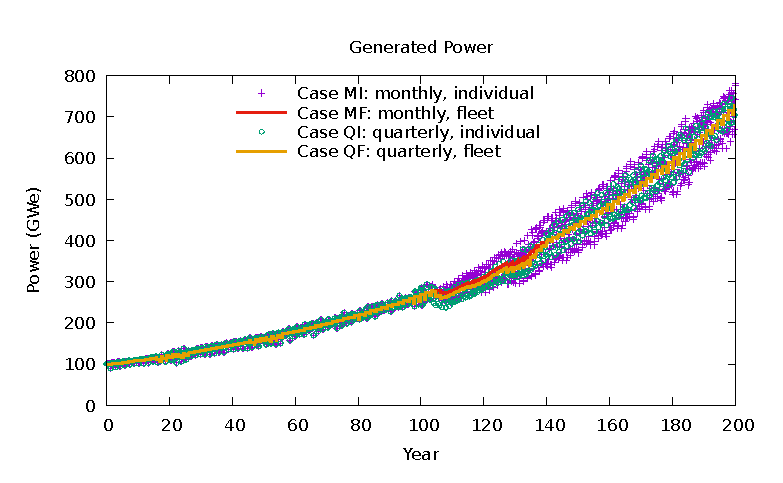
\includegraphics[width=1.0\textwidth]{exp2/power.eps}
    \caption[Generated power]{
        Generated power for all four cases.  A fuel shortage occurs from about
        year 100 to about year 140.  In cases MI and QI with individual reactor
        modeling, refueling cycles become much more synchronized during and
        after the fuel shortage resulting in large power fluctuations --- an artifact of the
        \emph{cycle staggering effect}.
    }
    \label{fig:power}
\end{figure*}

\begin{figure*}[!h]
    \centering
    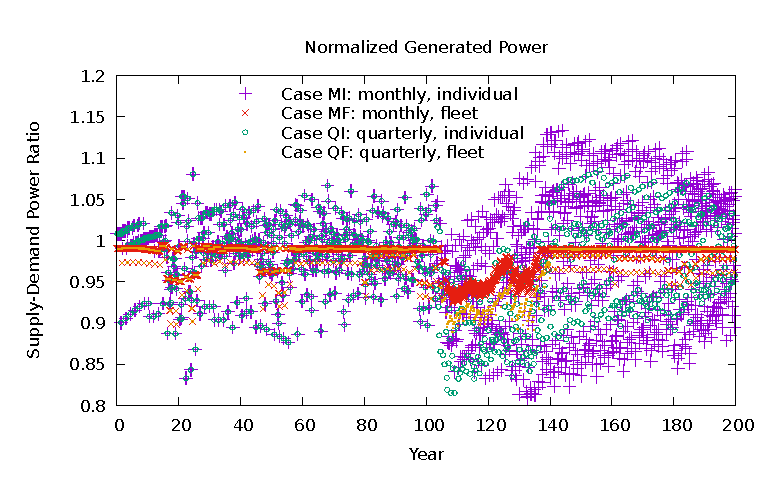
\includegraphics[width=1.0\textwidth]{exp2/power-rel.eps}
    \caption[Normalized power]{
        Generated power is normalized to the expected 1\% exponential growth
        curve for all four cases.  A fuel shortage occurs from about year 100
        to about year 140.  The \emph{cycle staggering effect} can be seen as
        excessive divergence above and below $1.0$ in cases MI and QI where
        the shortage increases cycle synchronization significantly. The
        \emph{quantized shutdown effect} causes part of the discrepancy
        between quarterly and monthly time steps for fleet reactor modeling
        (cases MF and QF) during the shortage; a longer time step causes more
        reactor outage than necessary. The consistent jumping up and down for
        the fleet reactor cases (even pre-shortage) is caused by the misalignment of reactors going
        offline (multiples of 12 months) and the build period (21 months).
    }
    \label{fig:power-rel}
\end{figure*}

\subsection{Fuel Shortage}

For the fleet reactors, fuel shortage is exactly the
difference between generated power and installed power capacity. Measuring the
fuel shortage for individual reactor cases, however, requires careful
accounting of the difference between reactors that are offline for a normal
refueling outage and reactors that are offline because they have insufficient
fuel. Equation \ref{eq:shortage} shows how this is calculated for cases MI and
QI.

\begin{equation}
    P_{outage}(t) = \sum\limits_{r \in R_t} P_r \cdot H[t-(\tau(t,r) + \Delta\;t_{out})] \cdot [1-O(t,r)]
    \label{eq:shortage}
\end{equation}

\noindent
where $R_t$ is the set of all reactors, $P_r$ is the power capacity of reactor
$r$, $H$ is the Heaviside function, $\tau(t,r)$ is the beginning of the most
recent refueling outage of reactor $r$ before $t$, $\Delta\; t_{out}$ is the
normal refueling outage duration, and $O(t,r)$ is 1 if reactor $r$ is
producing power at time $t$ and zero otherwise.

Figure \ref{fig:unfueled} shows the fuel shortage more explicitly for each of
the four cases with the case MI and QI results being the cumulative version of
Equation \ref{eq:shortage}.  The individual reactor modeling cases result in
more cumulative outage than corresponding fleet-based cases. The quarterly
time step of cases QI and QF also make the outage significantly more severe.
Cases MI and QI exhibit approximately twice as much offline power as their
corresponding fleet based simulations in cases MF and QF.  The monthly time
step simulations also have roughly twice as much offline power as their
corresponding quarterly cases.

\begin{figure}[!h]
    \centering
    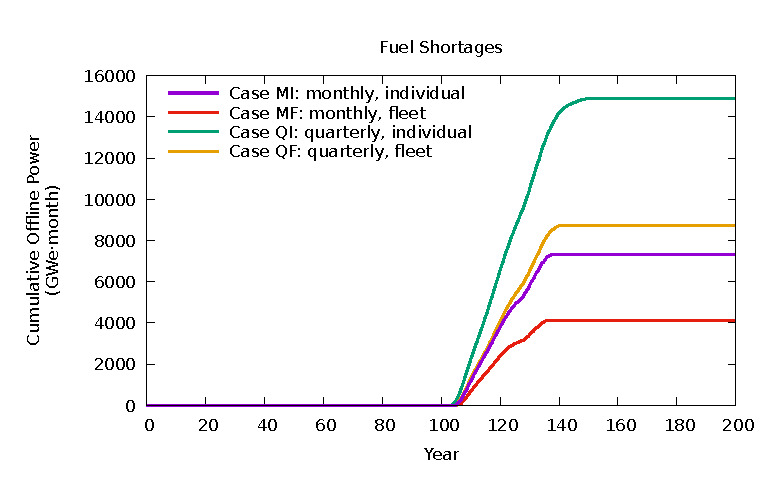
\includegraphics[width=1.0\columnwidth]{exp2/unfueled.eps}
    \caption[Cumulative offline power caused by fuel shortage]{
        Cumulative offline power for reactors that had delayed cycle start caused
        by fuel shortage. The difference between individual and fleet based
        modeling is primarily a result of the \emph{fuel sharing effect}. The
        difference between monthly and quarterly time steps is primarily
        a result of the \emph{inventory drawdown effect}.
    }
    \label{fig:unfueled}
\end{figure}

Quantifying imperfect fuel sharing is a bit difficult, but Figure
\ref{fig:badshare} provides one way to see the \emph{fuel sharing effect}
showing wasted batch-months computed using Equation \ref{eq:badshare}.  Fleet
reactor modeling, by design, exhibits perfect fuel sharing (zero
inefficiency) and so is not included in this figure.  Every batch that is
given to a reactor that ends up not being able to start its cycle at the
scheduled time (caused by fuel shortage) adds one to this cumulative total for each
time step the cycle start is delayed.

%% Paul Wilson says:
%%
%% What about a different measure of fuel sharing effect?  Perfect sharing
%% in a fleet reactor results in N_o reactors operating.  For individual
%% reactors, that would mean floor(N_o) reactors.  Can't we measure the
%% actual number of reactors that are operating, N_actual, and accumulate
%% floor(N_o) - N_actual as a measure of the effect of fuel sharing?  Would
%% this be substantially different?
%%
%% rwcarlsen responds:
%%
%% This could be interesting, but it is quantifying the significance of the
%% quantized shutdown effect discussed in the power production section of
%% results and doesn't belong here with the fuel sharing discussion - which is
%% only pseudo-related. Fuel sharing effects are when alternative sharing of
%% fuel between individual reactors could have resulted in different
%% online/offline capacity levels. These effects step on each other a tiny bit,
%% but I think it still makes much more sense to discuss/treat them separately.

One useful overestimate of the fuel sharing inefficiency is to assume every
one of the "wasted" batches could have been given to a reactor enabling it to
operate.  Multiplying each of these cumulative batches by the fast reactor power capacity
(i.e., 450 MWe) provides a way to compare fuel sharing inefficiency with the
overall fuel outage.  This results in a cumulative energy deficit caused by
poor fuel sharing of roughly 2,000 $\text{GWe} \cdot \text{months}$ and 6,600
$\text{GWe} \cdot \text{months}$ for cases MI and QI respectively.  These
approximations account for a significant portion of the difference between individual
and fleet cases in Figure \ref{fig:unfueled} suggesting that most of the
discrepancy in cumulative outage between fleet and individual modeling is
caused by inefficient fuel sharing in the individual reactor cases.

The poor fuel sharing exhibited in the individual reactor cases would not
occur if there were no new reactors being built during the shortage.
Previously operating reactors only ever need one batch - receiving only a
single batch allows them to operate.  Newly constructed reactors need multiple
batches in order to begin operation, and if they receive less than a full core
they cannot operate.  The real world doesn't necessarily optimize for fuel
sharing efficiency very cleanly. There are many factors that can affect
real-world fuel sharing outcomes.  A few include:

\begin{enumerate}

    \item Multiple fuel quanta comprise a single batch (i.e., multiple
        assemblies per batch). This functionality is natively supported in the
        individual reactor model.

    \item On-hand fresh fuel inventory maintained at reactors. This
        functionality is natively supported in the individual reactor model.

    \item Long-term fuel contracts between reactors operators and fuel
        suppliers.

\end{enumerate}

Having multiple assemblies per batch (item 1 above) will further degrade fuel
sharing efficiency.  Even reactors that are short only one batch could
potentially receive some fuel and still be unable to operate.  In order to
maintain optimal sharing, fresh fuel now needs to be sent in all-or-nothing
multi-assembly quanta with higher preference to reactors that need fewer
assemblies.  Spare fresh fuel inventory (item 2 above) will have the global
effect of increasing total shortage severity; on average more batches of fresh
fuel will be idling unused.  However, it can potentially reduce the frequency
of outages for individual reactors in some cases.

If they were to ever occur, real world fuel shortages would likely not result
in optimal fuel sharing. However, modeling these the causes of suboptimal fuel
sharing is probably best accomplished with a more direct, intentional approach
rather than as a modeling artifact as seen here in cases MI and QI.  One way to
alleviate the poor fuel sharing is to modify the individual reactor model to
adjust the preference value on requests for fresh fuel depending on how many
assemblies it needs to have a full core.  The more assemblies it needs, the
lower it will set its request preference.  This will have the effect of
allowing the DRE in Cyclus to prefer sending
fuel to reactors that need less to operate.

\begin{figure}[!h]
    \centering
    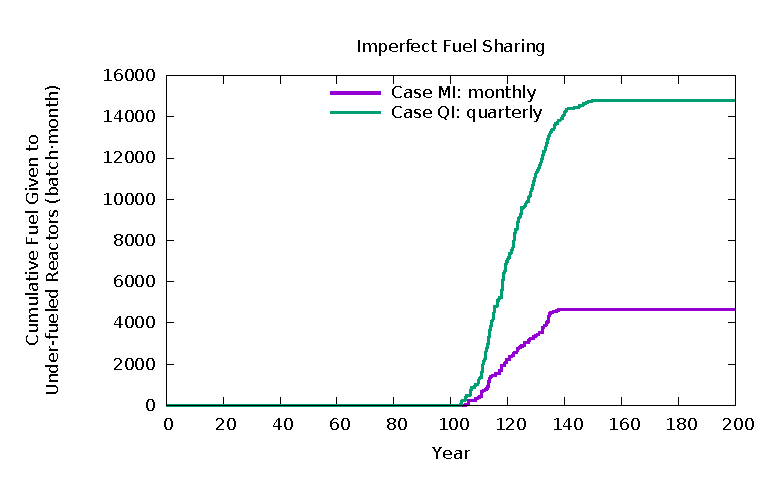
\includegraphics[width=1.0\columnwidth]{exp2/badshare.eps}
    \caption[Cumulative unnecessary idling fuel]{
        Fuel sharing inefficiency approximated by the cumulative number of
        fuel batches given to each reactor on each refueling period multiplied
        by the number of time steps that reactor had to delay the start of its
        next cycle (caused by fuel shortage).  Fleet reactors implicitly have perfect fuel
        sharing and so are not included here. The large difference
        between cases MI and QI is mostly a result of the \emph{inventory drawdown
        effect}. 
    }
    \label{fig:badshare}
\end{figure}

\subsection{Inventory Drawdown}

The large differences seen between monthly and quarterly time step cases in
Figures \ref{fig:unfueled} and \ref{fig:badshare} are primarily a result of the
\emph{inventory drawdown effect}.  Figure \ref{fig:puinv} helps to visualize
this effect.  The black dots in the figure represent impulse flows of
available Pu from fuel fabrication and into fast reactors.  Blue lines represent
the flows into Pu inventory available for making fuel. The in-flows are not
shown for the individual reactor cases because they are somewhat messy and
obscure other information in the plots. The other colored curves show Pu inventory
available for fabricating fast reactor fuel.  When the inventory curves meet and
force down the out-flows, fuel shortages occur.  While this is most clear for
cases MF and QF, the individual reactor scenarios (cases MI and QI) also have many
points during the shortage where the outflow point lies exactly on top of the
inventory point --- indicating that all available inventory is being
transferred.

Quarterly time steps have less frequent but larger impulse material flows.
The larger in-flows, however, do not compensate for the larger withdrawals
because facilities do not know about incoming inventory when they resolve
their outflow for a particular time step.  This information lag effectively
requires the floating Pu inventory to be maintained at a higher level during
the shortage.  This can be clearly seen in Figures \ref{fig:puinv} and \ref{fig:puinv-compare} where case QF has a higher
standing inventory than case MF during the fuel shortage years.  The case QF Pu
inventory is unable to drop below approximately 100 tonnes, which indicates
out-flows to be roughly equal to the Pu flow into inventory each time step
during those years.  This can be confirmed by the in-flow and inventory curves
touching at those points.  Case MF Pu inventory is similarly limited at about
the 30 tonne level.  As expected, the case QF withdrawals are also three times
higher than the case MF withdrawals, exactly matching the time step duration ratio
between the two cases.

Throughout most of the shortage, the aggregate outflow of Pu from separated
inventory is roughly the same in cases MF and QF.  However, because of the longer
time steps in case QF, the shortage starts slightly sooner because Pu inventory
must be maintained at a higher limit as described above.  The small difference
in outage start time has feedback effects.  Not only are extra reactors
offline, but those extra reactors are also discharging less aggregate spent
fuel for recycling.  This increases the discrepancy between the two
cases. Eventually the shortage in case MF ends slightly before it does in case
QF (shown most clearly in Figure \ref{fig:puinv-compare-zoom}). This feedback effect occurs because the reactors have a
conversion ratio greater than 1.0.

The horizontal striations visible in the monthly flows for case MI in Figure
\ref{fig:puinv} are a characteristic of the synchronization of reactor
refueling caused by the shortage.  A close-up view of these can be seen in
Figure \ref{fig:puinv-MI}. They begin at the end of the fuel shortage window
when many reactors come online together in groups and are resonances that the
inventory level jumps between.  This artifact is associated with poor cycle staggering
like that shown earlier in Figure \ref{fig:sync-cycle}.
These resonances gradually disappear as the
simulation progresses farther in time beyond the shortage and refueling cycles
become more staggered.

The in-flows shown for cases MF and QF show a periodic pulsing that begins
during the shortage in about year 120 and is shown in greater detail in Figure \ref{fig:puinv-MF}. This pulsing actually has nothing to
do with the shortage and is caused by the retirement of fast reactors.  The
first fast reactors are deployed in year 35 and have an 80 year lifetime.
When they retire, they discharge an entire core's worth of fuel rather than a
single batch.  After a 7-year cooling period, the first discharged full cores
begin to make it through the recycle loop in year 122.  Another interesting
feature visible in all four cases in Figure \ref{fig:puinv} is the minority
fraction of out-flow points that are higher than the bulk majority. These
higher out-flows occur once every 21 months when new reactors are built because
new reactors require a full core of fresh fuel rather than the single batch
needed when just refueling.  

\begin{figure*}[!h]
    \centering
    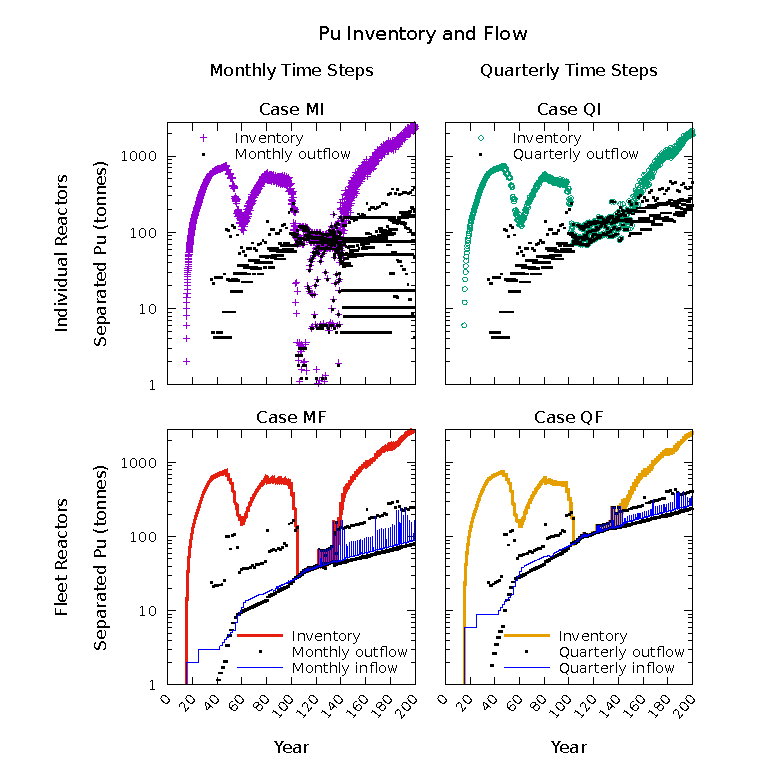
\includegraphics[width=1.0\textwidth]{exp2/puinv.eps}
    \caption[Separated Pu inventory and flow]{
        Separated Pu inventory and flows for all four cases.  In-flows for
        cases MI and QI are omitted because they are noisy and obscure other
        useful information.  When out-flows meet inventory, fuel shortages are taking place. A larger time step results in larger per time
        step material flows. These larger flows mean more material is not
        available for supplying to requesters.  This information lag causes
        more supply constraints than occur with smaller time steps -
        illustrating the \emph{inventory drawdown effect}. Another consequence of
        this effect is the larger standing Pu inventory during the shortage
        with larger time steps that can be seen in case QF than in case MF.
    }
    \label{fig:puinv}
\end{figure*}

\begin{figure*}[!h]
    \centering
    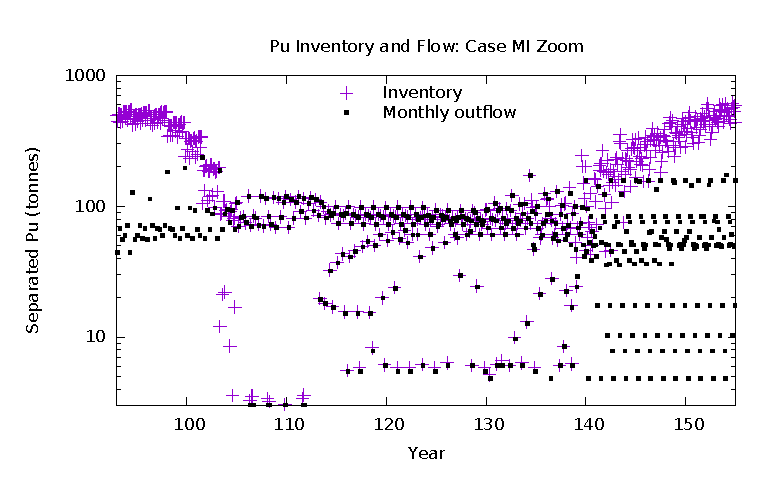
\includegraphics[width=1.0\textwidth]{exp2/puinv-MI.eps}
    \caption[Separated Pu inventory and flow: Case MI Zoom]{
        Zoom view of separated Pu inventory and flows from Figure \ref{fig:puinv} for case MI.  At locations where the
        outflow dots lie on/near the inventory level, fuel shortages are
        taking place.  This begins around year 105 and continues until about
        year 140 where Pu withdrawals become lower than standing inventory.
        The horizontal bands in out-flows starting around year 140 are caused
        by many previously offline reactors coming online together in groups.
        These fuel inventory level resonances gradually disappear as the
        simulation progresses.
    }
    \label{fig:puinv-MI}
\end{figure*}

\begin{figure*}[!h]
    \centering
    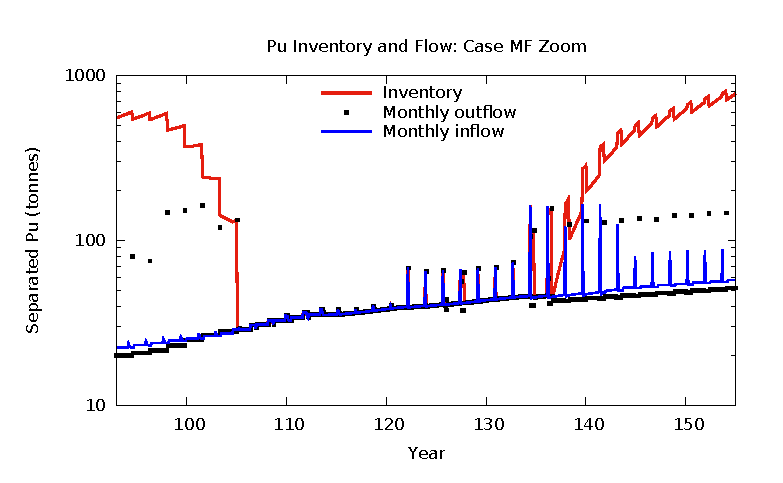
\includegraphics[width=1.0\textwidth]{exp2/puinv-MF.eps}
    \caption[Separated Pu inventory and flow: Case MF Zoom]{
        Zoom view of separated Pu inventory and flows from Figure \ref{fig:puinv} for case MF.  At locations where the
        outflow dots meet the inventory level, fuel shortages are taking
        place.  This begins around year 105 and continues until about year 140
        where Pu withdrawals become lower than standing inventory.  The
        periodic pulsing that begins just after year 120 is caused by the
        first fast reactor retirements; the first fast reactors deployed starting in
        year 35 retire annually after their 80 year lifetime and discharge an entire core's
        worth of fuel rather than the usual single batch for refueling.
    }
    \label{fig:puinv-MF}
\end{figure*}

Figure \ref{fig:puinv-compare} shows the same inventory curves from Figure
\ref{fig:puinv} superimposed. Perhaps counter-intuitively, lower separated
plutonium inventory during the shortage generally indicates fewer unfueled
reactors.  Lower inventory levels mean available Pu is being utilized more
efficiently rather than sitting idle.  Cases QI and QF with their longer time
steps show higher inventories indicating a more severe shortage.  Cases QI and
QF take longer to recover from the shortage and fall a bit behind with respect
to building up Pu stocks because of the delayed contributions of more unfueled
reactors to the separated Pu pool.  This can be seen most clearly in Figure
\ref{fig:puinv-compare-zoom}.  Cases MI and QF recover Pu inventory
post-shortage at about the same time and rate --- this is consistent with their
approximately equivalent cumulative offline power capacity curves in Figure
\ref{fig:unfueled}.

\begin{figure*}[!h]
    \centering
    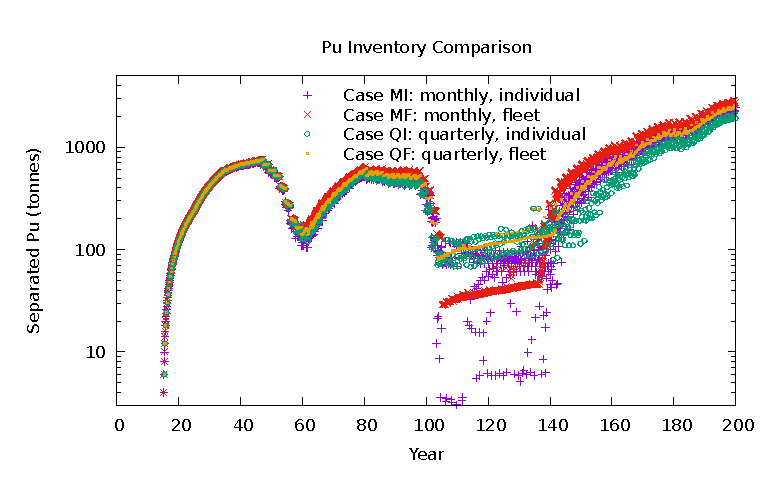
\includegraphics[width=1.0\textwidth]{exp2/puinv-compare.eps}
    \caption{
        Separated Pu inventories for all four cases.  Differences in modeling
        choices are not particularly significant until about year 100 when
        fuel shortages begin.  These differences gradually decay away starting
        in year 140 after fuel shortages have ebbed.
    }
    \label{fig:puinv-compare}
\end{figure*}

\begin{figure*}[!h]
    \centering
    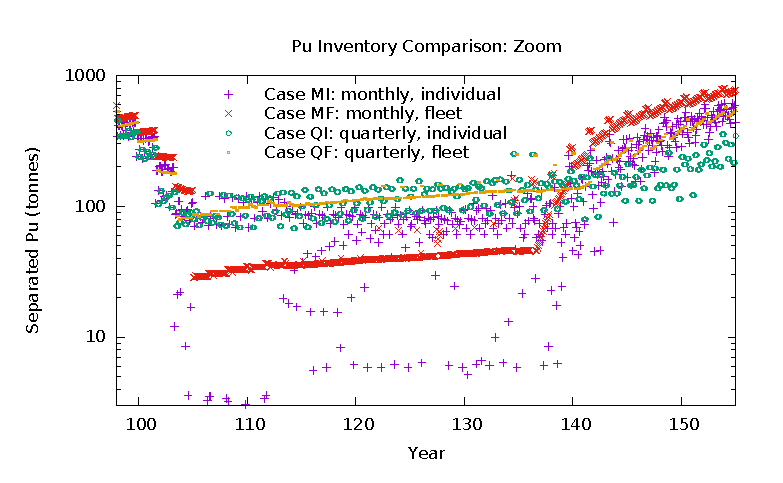
\includegraphics[width=1.0\textwidth]{exp2/puinv-compare-zoom.eps}
    \caption{
        Separated Pu inventories for all four cases zoomed in on the fuel
        shortage years.  Higher aggregate Pu inventory  during the shortage is
        correlated with both a longer shortage and a slower post-shortage
        recovery of Pu inventory.
    }
    \label{fig:puinv-compare-zoom}
\end{figure*}

The reactors in all the scenarios request fresh fuel only when they need it.
While this is an unrealistic behavior for real-world facilities, it is closer
to a globally optimum fuel management strategy.  Keeping on-hand fresh fuel
batches would also have the same effect of increasing idling Pu
quantities and would make the fuel shortage worse overall.

Also notable is that different modeling choices (e.g., time step duration,
facility discretization, etc.) may have varying levels of significance
depending on the scenario/context they are operating in.  As shown in Figure
\ref{fig:puinv-compare} before the fuel shortage begins, differences between
each of the four cases are relatively minor.  However, after the shortage
begins near year 100, separated Pu inventories vary much more significantly
between the different cases.

Raw data, custom code, instructions for reproducing results, and other
artifacts are available for download and use at
\url{http://dx.doi.org/10.6084/m9.figshare.1546775} \cite{Carlsen2015}.

\section{Conclusion}

Different modeling choices can have a significant impact on the outcome of a
simulation.  With discrete reactor modeling many factors must be considered in
order to ensure the integrity of conclusions.  Individual reactor outage
modeling can be very useful for certain analyses, but it can reduce result
quality if things such as cycle staggering are not handled appropriately.  The
fleet and discrete models used here are just two points in a multi-dimensional
spectrum of modeling choices. For example, if fuel sharing is of interest but cycle
staggering is not, individual reactors could be used with the power capacity
lowered and the outage reduced to zero duration, including the capacity factor
in the reactor's power capacity.

Modeling reactors individually can provide valuable insight not possible with
the fleet-based reactor modeling.  For example, bringing reactors back online
following shortage-induced outages should not necessarily follow the natural
pacing of fuel availability, otherwise refueling cycles become
unsatisfactorily synchronized.  If individual reactor modeling fidelity is not
required, then performance benefits in both simulation run time and data
analysis may suggest a fleet-based modeling approach.

Increasing time step duration increases facilities' standing inventory
requirement during supply constrained periods.  Here we observe a factor of
three difference between standing inventories of separated Pu for a large
portion of the simulation --- something certain analyses are very sensitive
to.  Facilities can provide no more inventory than they can hold on a single
time step.  So increasing time step duration for a facility with unconstrained
supply generally means higher standing inventories are required in order to
achieve equal throughput.  Facilities with large inventory buffer that are
unconstrained are not affected significantly by the time step duration when
operating in isolation.  However, even when facilities do not have individual
inventory or throughput limits, the time step can still have a significant
effect. The \emph{inventory drawdown effect} can impact the aggregate
throughput of supply-constrained recycle loops by affecting minimum bounds on
idling material quantities.

The impact of modeling assumptions depends heavily on the metrics of interest.
For example, someone interested in fuel-shortage driven reactor outages would
observe a factor of four span among the four cases shown in this comparison
exercise.  However, someone more interested in the overall transition
mechanics would not see as significant a discrepancy.  In an unconstrained
supply setting, varying the time step duration or discretization of facility
modeling has a smaller impact on the overall simulation results.
Differences become more significant in material constrained regimes.
Robustness in constrained regimes can be especially useful in the context of
sensitivity and optimization analysis.

The value of realism in fuel cycle modeling is greatly enhanced by an
associated understanding of how outcomes are affected by added fidelity.
Cyclus' flexibility for accommodating different modeling choices uniquely
enables many interesting comparisons.  Those in the field of fuel cycle
analysis in general should be cognizant of how modeling choices are affecting
results and conclusions through exercises like the one here.  Even if the
outcome is that a particular modeling decision has little impact on results,
efforts to measure and document these impacts can provide confidence in the
appropriateness of modeling choices, reducing the need to rely on intuition
for cycle analysis work.

\section{Acknowledgements}

This research is being performed in part using funding received from the DOE
Office of Nuclear Energy's Nuclear Energy University Programs.  The authors
thank the NEUP for its generous support.

\begin{center}
\includegraphics[width=1.5in]{neup_logo_large.jpg}
\end{center}

\pagebreak

%%%%%%%%%%%%%%%%%%%%%%%%%%%%%%%%%%%%%%%%%%%%%%%%%%%%%%%%%%%%%%%%%%%%%%%%%%%%%%%%
\bibliographystyle{ans}
\bibliography{refs}
\end{document}

